%!TEX root=Principal.tex
\chapter{CLASSIFICADOR BAYESIANO DO USUÁRIO}
\label{cap:proposta}
Após a especificação do projeto de IHR, onde definiu-se as características do ambiente, do robô utilizado e detalhes importantes do projeto como escopo e variáveis analisadas, realizou-se testes de interação para analisar informações que são importantes à criação do classificador do usuário. Este classificador utiliza técnicas bayesianas, mais especificamente, as redes bayesianas para incluir dependência entre as variáveis consideradas no projeto. Por ser um classificador estatístico, ele trabalha com a probabilidade da variável ser causada por um determinado efeito. No caso da tese, é a probabilidade de ser um determinado perfil dado a percepção que ele teve sobre as ações do robô. Essa classificação será importante para uma tomada de decisão direcionada ao perfil, durante a interação. Os passos para a criação do classificador são apresentados ao longo dessa seção e estão ilustrados através da figura~\ref{fig:construcao}.

\begin{figure}[ht!]
	\centering
	\begin{minipage}{\textwidth}
		\caption{Visão geral do processo de construção do classificador.}
		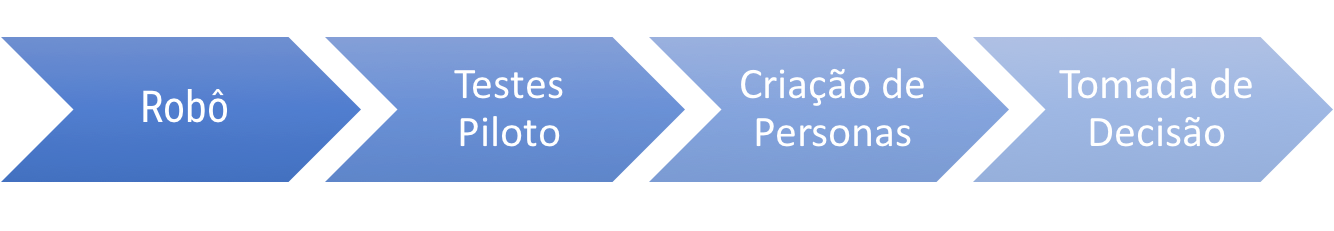
\includegraphics[width=\textwidth]{construcao.png}
		\smallcaption{Fonte: o autor.}
		\label{fig:construcao}
	\end{minipage}
\end{figure}

Os primeiros passos para a criação do classificador, blocos definidos na cor verde da figura~\ref{fig:construcao}, são as delimitações das variáveis de ações, que o robô executa na interação, a análise das respostas que auxiliaram, junto as heurísticas de avaliação de interface, a determinar novas variáveis ao contexto do robô. E por fim, a criação das Personas com o auxílio do algoritmo de agrupamento de dados QG-SIM. As Personas são as variáveies alvo do processo de classificação do perfil do usuário, já que elas conseguem aderir a um intervalo mais amplo de perfis.

Na sequência, os blocos em azuis, definem-se as variáveis que compõem a rede bayesiana, como foi determinada a estrutura da rede e as tabelas de probabilidades condicionais de cada variável ou nó da rede bayesiana. Depois, é descrito como é realizado a execução dos testes com a rede bayesiana. Finalizado, através de como essa classificação é utilizada durante a interação e o que é necessário realizar para identificar cada variável da rede, blocos em laranja. Inicia-se a definição dos limites das ações do robô na seção~\ref{sec:comportamento-robo}.

\section{Ações do Robô}
\label{sec:comportamento-robo}
A partir do robô construído para os experimentos (vide seção~\ref{sec:robo}), uma série de características consideradas auxiliam na interação social com ser humanos. Com base nos atuadores de interação existentes, foram mapeados as variáveis de ações do robô, que devem possuir seus valores limitados para que simplifique as tabelas de probabilidades condicionais do classificar bayesiano. A tabela~\ref{tab:variaveisvalores} apresenta as variáveis e a restrição do domínio de cada uma. Além das variáveis de ações do robô, algumas variáveis do cenário de interação também são consideradas, como o caso da posição e proximidade.

\begin{table}[!ht]
	\caption{Variáveis de Comportamento do Robô}
	\label{tab:variaveisvalores}
	\centering
	\begin{tabular}{c | c}
		\hline
		Variável & Valor \\
		\hline
		Gestos & curto \\
		& longo \\
		\hline
		Estilo da Fala & educada \\
		& autoritária \\
		\hline
		Expressão Facial & amigável \\
		& não amigável \\
		\hline
		Proximidade & longe - (Entre Pública e Social ) \\
		& perto - (Entre Pessoal e Íntima ) \\
		\hline
		Velocidade & rápida \\
		& devagar \\
		\hline
		Posição & sentado \\
		& em pé \\
		\hline
	\end{tabular}
	\smallcaption{Fonte: O autor.}
\end{table}

As variáveis da tabela~\ref{tab:variaveisvalores} são importantes, pois auxiliam a determinar o comportamento de reação do perfil do usuário para um mesmo tipo de ação do robô. Por exemplo, se o robô encontra-se próximo da pessoa, entre as zonas Pessoal e Íntima, um gesto com o manipulador com grande amplitude pode gerar um desconforto maior, do que o mesmo gesto ocorrendo entre as zonas Pública e Social. Outro cenário é a aproximação do manipulador próximo ao rosto do usuário, a reação é positiva ou negativa.

Alguns exemplos sobre os domínios das variáveis podem auxiliar a compreender quais são as ações correspondentes. Um exemplo para estilo de fala educada e autoritária são: ``Por favor, poderia me auxiliar a encontrar minha garrafa'' e ``Encontre minha garrafa'', respectivamente. Para ilustrar o domínio das expressões faciais é apresentada a figura~\ref{fig:dominioexpressoesfaciais}.

\begin{figure}[ht!]
	\centering
	\begin{minipage}{\textwidth}
		\caption{Visão geral do processo de construção do classificador.}
		\begin{subfigure}[b]{0.48\textwidth}
			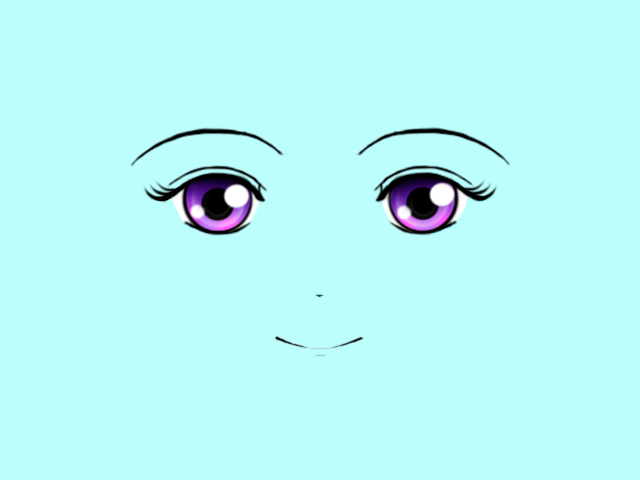
\includegraphics[width=\textwidth]{happy.png}
	        \caption{Feliz}
	        \label{fig:feliz}
	    \end{subfigure}
	    \hfill
		\begin{subfigure}[b]{0.48\textwidth}
	        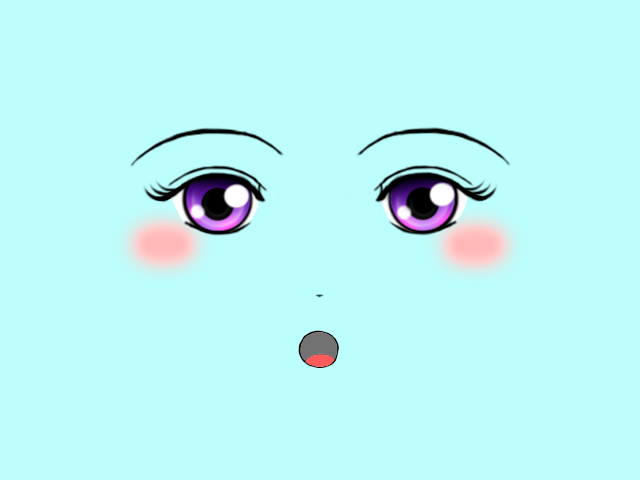
\includegraphics[width=\textwidth]{surprise.png}
	        \caption{Surpresa}
	        \label{fig:surpresa}
	    \end{subfigure}

		\begin{subfigure}[b]{0.48\textwidth}
	        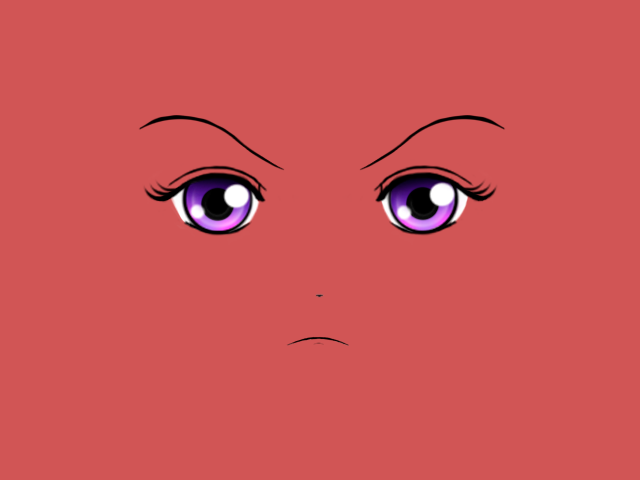
\includegraphics[width=\textwidth]{angry.png}
	        \caption{Nervosa}
	        \label{fig:nervosa}
    	\end{subfigure}
		\hfill
		\begin{subfigure}[b]{0.48\textwidth}
	        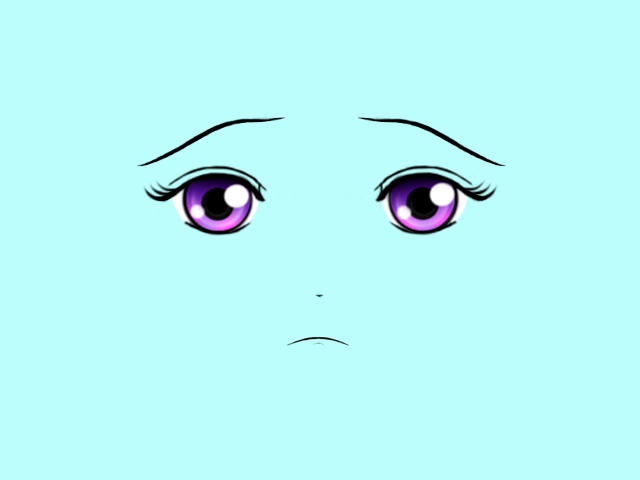
\includegraphics[width=\textwidth]{sad.png}
	        \caption{Triste}
	        \label{fig:triste}
    	\end{subfigure}
		\smallcaption{Fonte: o autor.}
		\label{fig:dominioexpressoesfaciais}
	\end{minipage}
\end{figure}

Nos exemplos apresentados na figura~\ref{fig:dominioexpressoesfaciais}, pode-se definir dentro do domínio da variável as figuras \ref{fig:feliz} e \ref{fig:surpresa} como expressões amigáveis e as figuras \ref{fig:nervosa} e \ref{fig:triste} como não amigáveis, dado os sentimentos que essas expressões representam. O programa que realiza a interação da face do robô foi desenvolvido em HTML e Javascript. Ele encontra-se disponível através do endereço \url{https://github.com/amasiero/robot_face}. Com o domínio das variáveis definidos, é necessário preparar as respostas dos questionários para o algoritmo de agrupamento e as heurísticas de avaliação de interface para verificar se elas auxiliam na classificação do perfil.

\section{Preparando as resposta dos questionários}
\label{sec:respostasbd}
Cada questionário (pré e pós teste) foi implementado utilizando a ferramenta on-line Google Forms~\footnote{https://docs.google.com/forms/u/0/}. Nessa ferramenta as respostas são armazenadas em planilhas eletrônicas, ficando assim separadas as respostas entre os dois questionários. Os questionários foram apresentados nas seções~\ref{sec:questionariopreteste} e \ref{sec:questionarioposteste} É necessário unificá-los para auxiliar na identificação dos perfis dos usuários. Além disso, o algoritmo de agrupamento trabalha com uma base de dados única. Para fazer esse processo de unificar as bases de dados, criasse um arquivo csv (\emph{comma-separated values}) e uni na mesma linha os registros que possuem o mesmo identificador do questionário pré e pós teste. O arquivo csv gerado serve para realizar análise dos dados e para criação dos grupos de perfis que são responsáveis pela composição das Personas. A composição de Personas representa o conjunto de variáveis que fazem parte do resutaldo nas consultas do classificador bayesiano implementado.

\section{Heurísticas de Interação Humano-Robô}
\label{sec:heuristicas}
Avaliação heurística é um método utilizado por especialistas em usabilidade para verificar problemas de interação em interfaces de sistemas e produtos. \citeonline{nielsen:1994} apresenta 10 heurísticas para avaliações de interfaces em sistemas web (vide seção~\ref{sec:avaliacao}). As heurísticas de Nielsen tem sido amplamente utilizadas ao longo dos tempos para sites e sistemas desktop. Alguns trabalhos discutidos ao longo da seção~\ref{sec:ihrux} apresentam modificações das heurísticas de Nielsen para o cenário de interação humano-robô.

Nos questionários pré e pós teste preenchido pelos usuários, notou-se que apontavam no robô a falta ou a presença de características que representavam as heurísticas de avaliação. Cada usuário dava mais atenção a determinadas características, que compunham diferentes perfis de interação. Assim, as heurísticas de avaliação apresentadas pela literatura foram estudadas. A partir desse estudo, verificou-se que as heurísticas mais presentes nos comentários dos usuários, também estavam presentes nas listas contidas na literatura. Dentre as heurísticas que apresentam uma descrição de maior aplicabilidade em robótica social e interação humano-robô estão as heurísticas de \citeonline{clarkson:2007} (vide tabela~\ref{tab:heuristicasihr}).

Nesse momento é realizado a seleção das heurísticas em comum com os comentários dos usuários. Essas heurísticas são transformadas em variáveis que compõem a rede bayesiana, a fim de auxiliar na classificação do perfil do usuário em interação. Com base nas observações e comentários dos testes de interação, mais os estudos da literatura, foi possível identificar as seguintes heurísticas para transformá-las em variáveis que formam o conjunto de classificação do usuário:

\begin{itemize}
	\item Visibilidade do estado do sistema;
	\item Uso de sugestões naturais;
	\item Síntese do sistema e interface;
	\item Ajudar o usuário a reconhecer, diagnosticar, e recuperar de erros.
\end{itemize}

Cada uma das heurísticas apresentadas na lista acima, foram observadas durante os testes e possuem dependência condicional com os perfis e/ou com as ações do robô.

\section{Agrupando perfis com o algoritmo QG-SIM}
\label{sec:preparacao}
A partir da base de dados criada com as informações dos questionários, deve-se remover as informações de texto livre, uma vez que o algoritmo não possui um interpretador semântico. Sem o interpretador semântico, não é possível criar um modelo quantitativo para as respostas, onde exista uma significância comparativa.

As informações existentes nos questionários podem ser quantificadas, por exemplo a idade do usuário. A comparação de similaridade entre duas idades pode ocorrer com medidas de distância, por exemplo, a distância euclidiana. Outras medidas também podem ser aplicadas, porém dependerá do tipo de informação e necessidade do projeto~\cite{masiero:2013}. No caso do agrupamento de perfis desta tese, para informações numéricas, a distância euclidiana é adotada. Ela atende a necessidade do algoritmo e do processo para agrupamento dos perfis.

Variáveis categóricas, ou seja, as variáveis que possuem um valor textual que podem ser separadas em categorias, deve-se realizar um tratamento para quantifíca-las. Existem duas opções para quantificar as variáveis categóricas. A primeira opção é inserir um código númerico para cada valor, por exemplo, os valores ``Celular, Computador, Tablet, Autoatendimento, Caixa Físico'' recebem um valor representado por um número inteiro cada ficando ``Celular = 1, Computador = 2, Tablet = 3, Autoatendimento = 4, Caixa Físico = 5'', conforme~\citeonline{masiero:2013}. A segunda opção é transformá-las em variáveis \emph{dummies}~\footnote{http://pandas.pydata.org/}. O método \emph{dummies} transforma cada opção de resposta ou cada categoria em uma nova variável binária onde o valor 1 é para quando a opção for verdadeira e 0 para o oposto.

Realizado os procedimentos para quantificar todas as variáveis, a base de dados já pode ser inserida no algoritmo para o processo de agrupamento. Porém, um outro detalhe nos dados é importante para evitar o problema de tendência no algoritmo. Cada variável possui uma escala diferente. Essa diferença na escala das variáveis pode gerar as tendências no resultado do algoritmo. Assim, é necessário padronizar os valores númericos existentes na base dentro da mesma escala. Para realizar a padronização dos dados o processo de normalização é executado. A normalização mais comum a ser feita é manter os valores das variáveis entre 0 e 1~\cite{lattin:2011}. A equação~\ref{eq:normalizacao1} apresenta a forma mais simples de realizar o processo de normalização dos dados. É feita a divisão do valor da característica pelo valor máximo encontrado entre a característica analisada.

\begin{equation}
	X_{i_{normalizado}} = \frac{X_i}{\max_{X_i}}
	\label{eq:normalizacao1}
\end{equation}

Entretanto, o uso da equação \ref{eq:normalizacao1} para normalizar os dados, pode gerar também uma tendência ou generalização da normalização. Pode existir uma concentração dos dados em um determinado intervalo generalizando a informação coletada~\cite{masiero:2013}. Para evitar o problema da concentração dos dados, utiliza-se a equação \ref{eq:normalizacao2} como método mais efetivo na normalização dos dados.

\begin{equation}
	X_{i_{normalizado}} = \frac{X_i - \min_{X_i}}{\max_{X_i} - \min_{X_i}}
	\label{eq:normalizacao2}
\end{equation}

Após o processo de normalização, as escalas da base estão com uma distribuição uniforme e prontas para serem consumidas pelo algoritmo. O processo de normalização é executado internamente no algoritmo, para evitar esse tipo de problema no agrupamento.

Com as informações normalizadas, o próximo passo é executar o algoritmo de agrupamento QG-SIM. A implementação do algoritmo pode ser encontrada no endereço \url{https://github.com/amasiero/qgsim}. O algoritmo solicita um paramêtro de entrada para auxiliar na construção dos grupos. Esse parâmetro é chamado de valor de similaridade. O valor de similaridade atende um intervalo de 0.0 até 1.0, sendo 0.0 sem similaridade e 1.0 com total similaridade. O nome dado a esse parâmetro é valor Q. O valor Q determina quais perfis pertencerão ao mesmo grupo~\cite{masiero:2013}.

O QG-SIM tem um diferencial dos demais algoritmos que auxilia na construção de Personas. Ao realizar o processo de agrupamento, o QG-SIM garante que a similaridade mínima entre todos os elementos do grupo é igual ao informado no valor Q. Esse comportamento garante uma homogeneidade entre os perfis agrupados, auxiliando no alcance das Personas construídas ao maior número de pessoas~\cite{masiero:2013}.

A execução foi realizada com três valores Q diferentes, 0.6, 0.7 e 0.8. Após cada execução é verificado como foi realizado o agrupamento, para que não existam grupos muito generalizados e nem grupos muito especializados. Para o valor $Q = 0.6$, foram encontrados 3 grupos, dois grupos com 1 pessoa cada e um grupo contendo os demais perfis. Ficou muito generalizado. O próximo valor testado foi de $Q = 0.8$. Nesse caso, o resultado foi muito especifíco, pois houve 9 grupos sendo grande parte com 1 ou 2 perfis e poucos grupos com 5 perfis. O valor intermediário $Q = 0.7$, apresentou um comportamento melhor onde encontrou 5 grupos. 2 grupos com 1 perfil cada, 1 grupo com 7, outro com 9 e o maior com 21. Alguns fatores, como idade, redes sociais, contato com robôs, entre outros foram determinantes para esse resultado. Detalhes sobre cada grupo é apresentado no capítulo~\ref{cap:resultados}. Agora que os grupos estão definidos, deve-se criar as Personas que representam cada um deles. A criação das Personas é apresentada na seção~\ref{sec:criacaopersonas}, a seguir.

\section{Criação das Personas}
\label{sec:criacaopersonas}
Assim que os grupos são definidos, utiliza-se medidas de tendência central para obter um valor comum ao grupo para cada variável utilizada pelo QG-SIM durante o agrupamento dos perfis. As medidas de dispersão mais comuns são: média, mediana e moda. A aplicação de cada uma depende do tipo de informação que contém nas variáveis da base de dados. Informações númericas, por exemplo, podem ser utilizadas medidas como a média ou a mediana. Para dados categóricos, o mais indicado é que utilizem a medida de tendência central moda, pois ela identifica o valor pela opção mais frequente nas respostas~\cite{masiero:2013}.

Os valores obtidos em cada uma das variáveis auxiliam no processo de construção da Persona. Elas são responsáveis pela definição dos valores sobre idade, o uso de óculos, tipo do cabelo, gênero, e outras informações que caracterizam o perfil. Nesse momento, as características que constroem as Personas estão definidas. O próximo passo é construir as experiências da Persona, descrever comportamentos e experiências de vida dela. Para isso, utiliza-se as informações de texto livres preenchidas nos questionários. São realizadas análises sobre as respostas e identifica os pontos em comum entre os perfis do grupo. Os pontos em comum são utilizados como base para construir a história da Persona. A história da Persona deve trazer características importantes ao modo como ela interage com o sistema, no caso o robô. As Personas são importantes, pois garantem que uma ampla quantidade de perfis seja contemplado em cada uma delas. Elas auxiliam na generalização dos processos para definir as interações entre os perfis.

Cinco Personas foram construídas. Essas são apresentadas nas tabelas~\ref{tab:joaquim}, \ref{tab:mariaeduarda}, \ref{tab:alfredo}, \ref{tab:danielo} e \ref{tab:manuel}, a seguir.

\begin{table}[!ht]
	\caption{Persona Joaquim}
	\label{tab:joaquim}
	\centering
	\begin{tabular}{ m{2 cm} | m{13cm} }
		\hline
		Foto: & \rule{0cm}{2.7cm} 
\includegraphics[scale=0.8]{joaquim.png} \\
		\hline
		Nome: & Joaquim \\
		\hline
		Descrição: & Tem 21 anos, 1,71 m de altura, em geral não é uma pessoa séria ou carrancuda, mas também não é sorridente. É um homem \textbf{sociável}, cheio de amigos a sua volta e adora ir ao barzinho com eles. Mora na capital paulista, centro econômico brasileiro, local perfeito para um homem que gosta de variedade cultural. \textbf{Não fica longe de seu smartphone e também sempre que pode, está com seu laptop no colo navegando pelo Facebook e postando fotos no Instagram}. Tudo que pode ser resolvido pelo seu smartphone ele faz, seja por chamada de voz ou qualquer aplicativo. Mas, ainda não conseguiu se habituar aos serviços financeiros digitais, prefere o método clássico para guardar seu dinheiro, o colchão. Nunca viajou para fora do Brasil, inclusive seu mapa de viagens nacionais também não é extenso. Ao todo, visitou apenas 9 cidades do Brasil com o passar do tempo.

		Na universidade acompanhou os times de robótica nas competições e teve contato com diversos tipos de robôs, como os parecidos com humanos e animais, com mobilidade através de rodas e também os de linha de produção. Quando perguntam sua expectativa sobre robôs convivendo em sua casa, ele diz que tudo bem, desde que ele execute as \textbf{tarefas domésticas sempre com obediência e de certa maneira, também espera que o robô seja afetivo na interação}. Um comportamento próximo ao de uma diarista na família. Já no ambiente industrial, Joaquim acredita que os robôs são apenas ferramentas de trabalho e não devem fazer nada além de executar o que lhe foi programado. \\
		\hline
	\end{tabular}
	\smallcaption{Fonte: O autor.}
\end{table}

\begin{table}[!ht]
	\caption{Persona Maria Eduarda}
	\label{tab:mariaeduarda}
	\centering
	\begin{tabular}{ m{2 cm} | m{13cm} }
		\hline
		Foto: & \rule{0cm}{2.7cm} 
\includegraphics[scale=0.8]{maria_eduarda.png} \\
		\hline
		Nome: & Maria Eduarda \\
		\hline
		Descrição: & Aos 36 anos, com 1,71 m de altura, é uma garota reservada que adora sorrir em diversas ocasiões. É \textbf{bem sociável, e mantém os amigos por perto}. É uma mulher moderna e gosta de manter seu corte de cabelo mais curto que o convencional. Mora em São Bernardo do Campo, cidade da grande São Paulo e gosta muito de visitar o interior de São Paulo para passar seus feriados prolongados. Não vive sem seu celular, e no trabalho o computador é sua principal ferramenta. Quando está em \textbf{casa utiliza sua Smart TV para assistir suas séries e filmes favoritos}. Gostaria muito de ter um leitor de e-book para evitar carregar livros pesados durante seu trajeto pelo transporte público. Mesmo com essa adoção a tecnologia, empresas digitais, principalmente do mercado financeiro, não a atraem. Sempre \textbf{conectada através do celular, ela posta tudo no Facebook, tanto de trabalho quanto de lazer}.

		Já viajou algumas vezes para os EUA, sempre a passeio com o principal destino a Disney. Pelo Brasil, já viajou para algumas cidades fora de São Paulo e deixou sua marca por todas as regiões do país. Como ela trabalha em uma universidade de engenharia, já viu diversos tipos de robôs, que são utilizados nas aulas. Porém, nunca teve um contato direto com eles, a não ser seu aspirador de pó. Tanto em casa quanto no trabalho, ela espera que \textbf{robôs sejam capazes de realizar tarefas com eficácia, como dirigir um carro, digitar planilhas, mas que ao mesmo tempo não seja capaz de substituí-la}.\\
		\hline
	\end{tabular}
	\smallcaption{Fonte: O autor.}
\end{table}

\begin{table}[!ht]
	\caption{Persona Alfredo}
	\label{tab:alfredo}
	\centering
	\begin{tabular}{ m{2 cm} | m{13cm} }
		\hline
		Foto: & \rule{0cm}{2.7cm} 
\includegraphics[scale=0.8]{alfredo.png} \\
		\hline
		Nome: & Alfredo \\
		\hline
		Descrição: & Aos 24 anos, rapaz de estatura normal, por volta de 1,75m, está sempre com um belo sorriso no rosto, faça chuva ou faça sol. Sempre \textbf{tem pessoas a sua volta, gosta de contar piadas e fazer todos sorrirem}. Morador da cidade de São Bernardo do Campo, mas sempre que pode vai para o litoral paulista visitar os pais e curtir uma praia. Usa computador para fazer os trabalhos da faculdade e \textbf{passa grande parte do seu tempo no celular}. Não possui serviços financeiros digitas, pois ainda não conseguiu a aprovação do cadastro. Quando se trata de internet banking, \textbf{acredita que o seu computador é mais seguro que o uso de celular}.

		Alfredo vive antenado nas redes sociais, como Twitter, Instagram e Facebook. Ajudam ele a ficar conectado com as últimas notícias e eventos a sua volta. Tem um sonho de viajar para o exterior, mas isso ainda não foi possível, em compensação pelo Brasil já visitou mais de 30 cidades, a maioria na região Sudeste. Na universidade, através do curso de engenharia de automação, teve contato com robôs de fábrica e móveis conforme os laboratórios das disciplinas ocorriam. Quando perguntam a Alfredo o que ele espera de um robô doméstico e também um robô no trabalho, ele diz que \textbf{robôs devem executar as tarefas propostas de maneira eficiente e que seu interação seja toda por comando de voz}.\\
		\hline
	\end{tabular}
	\smallcaption{Fonte: O autor.}
\end{table}

\begin{table}[!ht]
	\caption{Persona Danielo}
	\label{tab:danielo}
	\centering
	\begin{tabular}{ m{2 cm} | m{13cm} }
		\hline
		Foto: & \rule{0cm}{2.7cm} 
\includegraphics[scale=0.8]{danielo.png} \\
		\hline
		Nome: & Danielo \\
		\hline
		Descrição: & Com 27 anos de idade, 1,83m, Danielo está sempre na \textbf{academia para treinar com seus amigos}. Mora em São Bernardo do Campo, e utiliza seu computador para fazer seu trabalho e o celular para manter contato com seus amigos. \textbf{Nunca quis saber de leitores de e-book, pois acha sua tecnologia sem utilidade nos dias atuais}. A sua única rede social é o Facebook. Ele acha que já toma tempo o suficiente e não precisa de outras para ver a mesma coisa. Danielo é um rapaz que já viajou bastante. Já visitou 3 países latinos e no Brasil visitou mais de 90 cidades, concetradas em sua grande parte, na região Sudeste. O contato com robôs é limitado e restrito a robôs de fábrica. Em casa \textbf{ele acredita que o robô será parecido com seres humanos para fazer as atividades domésticas, e no trabalho substituirão seres humanos em trabalhos repetitivos}, como nas fábricas e linha de produção.\\
		\hline
	\end{tabular}
	\smallcaption{Fonte: O autor.}
\end{table}

\begin{table}[!ht]
	\caption{Persona Manuel}
	\label{tab:manuel}
	\centering
	\begin{tabular}{ m{2 cm} | m{13cm} }
		\hline
		Foto: & \rule{0cm}{2.7cm} 
\includegraphics[scale=0.8]{manuel.png} \\
		\hline
		Nome: & Manuel \\
		\hline
		Descrição: & Aos 33 anos, 1,85 m,  Manuel um professor universitário sempre sorridente. Seus alunos sempre o procuram para esclarecer dúvidas e pedir conselhos. Mora em São Bernardo do Campo, próximo ao seu local de trabalho, por que adora o conforto de ir em sua casa poder almoçar uma comida fresca. Acredita que tem uma melhor qualidade de vida assim. \textbf{Não é muito fã de tecnologia de ponta, então fica contente em ter seu computador, onde resolve tudo que pode. Digitalmente, considera-se antisocial e não mantém cadastro em nenhuma rede social}.

		Já visitou paises pela Europa, África, América do Norte e do Sul. No Brasil, seu foco de visitar está na região Sudeste, principalmente o estado de Minas Gerais. No total já percorreu mais de 62 cidades pelo país. Como professor, sua linha linha de pesquisa principal de estudos é a robótica, fazendo com que tenha contato com todos os tipos de robôs. \textbf{Em casa, pensa em ter um robô para atender suas necessidades}, assim como no trabalho. Porém, o robô \textbf{no trabalho deve atender também as necessidades e expectativas da empresa}.\\
		\hline
	\end{tabular}
	\smallcaption{Fonte: O autor.}
\end{table}

As Personas apresentadas nas tabelas~\ref{tab:joaquim}, \ref{tab:mariaeduarda}, \ref{tab:alfredo}, \ref{tab:danielo}, \ref{tab:manuel} ajudaram na definição das independências condicionais entre as variáveis da rede bayesiana. Mais informações das análises feitas com base nas Personas, e também sobre sua criação, em relação a interação com o robô são apresentadas no capítulo~\ref{cap:resultados}.

\section{Selecionando e estruturando variáveis como rede bayesiana}
\label{sec:rede-bayesiana}
Neste momento todos os passos necessários para identificar as Personas, ações do robô e as necessidades do projeto foram realizados. As últimas variáveis selecionadas para compor a rede bayesiana para classifição do perfil do usuário, representado pela Persona, são as comportamentais. As variáveis comportamentais neste ponto estão ligadas as possíveis experiências que o usuário pode sentir na interação. Dentre as variáveis apresentadas na seção~\ref{sec:reacoes} são selecionadas as variáveis conforto e medo. As duas variáveis conseguem representar grande parte das demais variáveis comportamentais apresentadas. Neste momento, a forma de identificar as variáveis de conforto e medo, é através da declaração do usuário durante o teste e também nas respostas do questionário pós teste. A partir desse ponto, têm-se todas as variáveis definidas e é necessário definir a estrutura da rede bayesiana. Na sequência será apresentado cada conjunto de nós e suas dependências condicionais para a criação da estrutura da rede bayesiana de classificação, dado as especificações do projeto de IHR apresentado no capítulo~\ref{cap:projetoihr}.

Os nós raizes da rede bayesiana são compostos pelas 5 Personas apresentadas na seção~\ref{sec:criacaopersonas}. Elas são escolhidas como raiz por que representam os perfis de usuários que devem ser classificados durante a aproximação do robô. A probabilidade do usuário em interação ser ou não aquela Persona é determinada, pela quantidade de pessoas que pertencem ao grupo encontrado pelo QG-SIM. Como são nós raizes, não existem nenhuma evidência para compor seu valor de probabilidade, apenas a quantidade de pessoas de cada grupo. As equações~\ref{eq:joaquim}, \ref{eq:mariaeduarda}, \ref{eq:alfredo}, \ref{eq:danielo} e \ref{eq:manuel} representam a probabilidade de cada uma das Personas obtidas.

\begin{equation}
	\label{eq:joaquim}
	P(joaquim)
\end{equation}

\begin{equation}
	\label{eq:mariaeduarda}
	P(maria\_eduarda)
\end{equation}

\begin{equation}
	\label{eq:alfredo}
	P(alfredo)
\end{equation}

\begin{equation}
	\label{eq:danielo}
	P(danielo)
\end{equation}

\begin{equation}
	\label{eq:manuel}
	P(manuel)
\end{equation}

As variáveis são nomeadas com letras minúsculas, pois são variáveis com apenas dois valores representando ser ou não ser. Essa notação segue a convenção apresentada por \citeonline{russell:2002}.

Seguindo com a construção da rede, cada nó interno foi considerado com base nas variáveis criadas a partir das heurísticas de IHR, das ações do robô e também do contexto de uso e ambiente de teste. As independências condicionais entre cada nó foi observado pelos comentários de cada usuário durante os testes. O processo de criação dos nós é detalhado na sequência. A inclusão dos nós é feita com base nas variáveis apresentadas na tabela~\ref{tab:variaveisvalores}.

O nó Proximidade leva em consideração os espaços sociais definidos por \citeonline{hall:1969}. O domínio foi simplificado para \{perto, longe\}, pois durante os testes pilotos a reação do usuário era a mesma entre as regiões íntima e pessoal (perto) e as regiões social e pública (longe). A dependência condicional foi aplicada de acordo com a declaração explícita entre os perfis que sentiram algum desconforto com a aproximação do robô. A equação~\ref{eq:proximidade} define o cálculo de probabilidade condicional para a variável aleatória Proximidade.

\begin{equation}
	\label{eq:proximidade}
	P(proximidade | joaquim, alfredo, danielo)
\end{equation}

A próxima variável aleatória inserida é a Posição da pessoa no ambiente. O domínio dessa variável é determinado por \{sentado, em pé\}. Ela foi observada durante a prova de reconhecimento de pessoas e aproximação do robô na RoboCup de 2016. Nesse cenário, as pessoas que estavam sentadas ficavam bem desconfortáveis com a aproximação do robô, principalmente com relação ao seu manipulador. Nos teste pilotos, a situação demonstrou-se a mesma. As pessoas que estavam sentadas demonstravam um comportamento mais apreensivo do que as em pé. A equação~\ref{eq:posicao} apresenta o cálculo de probabilidade condicional para a variável Posicao.

\begin{equation}
	\label{eq:posicao}
	P(posicao | joaquim, maria\_eduarda, alfredo, danielo, manuel)
\end{equation}

As 4 próximas variáveis aleatórias descritas são referentes a ações do robô. Todos os 4 conjuntos são importantes na interação social e geram diferentes reações aos perfis de usuários. Um ponto interessante a ser resaltado é que cada Persona mapeada, ficou atenta durante a interação em apenas algumas das variáveis. As 4 variáveis são Expressão Facial (equação~\ref{eq:face}), Gestos (equação~\ref{eq:gestos}), Estilo da Fala (equação~\ref{eq:fala}) e Velocidade (equação~\ref{eq:velocidade}). Seus respectivos domínios estão descritos na tabela~\ref{tab:variaveisvalores}.

\begin{equation}
	\label{eq:face}
	P(face | joaquim, maria\_eduarda, alfredo, danielo, manuel)
\end{equation}

\begin{equation}
	\label{eq:gestos}
	P(gestos | maria\_eduarda, alfredo, danielo, manuel)
\end{equation}

\begin{equation}
	\label{eq:fala}
	P(fala | joaquim, alfredo, danielo, manuel)
\end{equation}

\begin{equation}
	\label{eq:velocidade}
	P(velocidade | joaquim, maria\_eduarda)
\end{equation}

A partir da variável Gestos, observou-se que quando ocorreu o toque do robô na pessoa, gerou uma situação de medo. A variável toque é mapeada com a dependência condicional da variável Gestos (equação~\ref{eq:toque}). Seu domínio é binário, $\{toque, \neg toque\}$.

\begin{equation}
	\label{eq:toque}
	P(toque | gestos)
\end{equation}

Cada heurística apontada na seção~\ref{sec:heuristicas} gerou um nó que representa uma variável aleatória da rede bayesiana. Todas as heurísticas utilizadas, possuem relação com os comportamentos do robô durante os testes de interação e também com as informações feitas pelos usuários. A lista a seguir mostra as heurísticas e as nomeações como variáveis aleatórias da rede bayesiana.

\begin{itemize}
	\item Visibilidade do estado do sistema - estado\_robo (equação~\ref{eq:estadorobo});
	\item Uso de sugestões naturais - natural (equação~\ref{eq:natural});
	\item Síntese do sistema e interface - sintese (equação~\ref{eq:sintese});
	\item Ajudar o usuário a reconhecer, diagnosticar, e recuperar de erros - ajudar (equação~\ref{eq:ajudar}).
\end{itemize}

\begin{equation}
	\label{eq:estadorobo}
	P(estado\_robo | joaquim, alfredo, manuel)
\end{equation}

\begin{equation}
	\label{eq:natural}
	P(natural | fala, gestos)
\end{equation}

\begin{equation}
	\label{eq:sintese}
	P(sintese | fala)
\end{equation}

\begin{equation}
	\label{eq:ajudar}
	P(ajudar | maria\_eduarda, alfredo)
\end{equation}

Por fim, são definidas as variáveis aleatórias chamadas de nós folhas da rede bayesiana. Esses nós correpondem ao sentimento das pessoas durante a interação com o robô. Esses sentimentos são declarados pelas pessoas durante a interação de acordo com o comportamento do robô. A composição das relações com esses nós foi dada pela observação dos testes e também das declarações realizadas através do questionário pós interação. As três variáveis aleatórias são conforto~\ref{eq:conforto}, desconforto~\ref{eq:desconforto} e medo~\ref{eq:medo}.

\begin{equation}
	\label{eq:conforto}
	P(conforto | proximidade, face, estado\_robo, natural, sintese)
\end{equation}

\begin{equation}
	\label{eq:desconforto}
	P(desconforto | posicao, face, estado\_robo, ajudar, natural)
\end{equation}

\begin{equation}
	\label{eq:medo}
	P(medo | velocidade, face, toque)
\end{equation}

As variáveis conforto e desconforto estão separadas, pois em alguns casos existiram pequenas diferenças que em uma mesma ação do robô, alguns usuários sentiram conforto e desconforto ao mesmo tempo. Por exemplo, ao se aproximar o robô chegou muito perto o que gerou o desconforto já que o usuário estava sentado, mas a expressão facial apresentada pelo robô no momento deixou ele tranquilo e confortável, mesmo não tendo como escapar da frente do robô (vide capítulo~\ref{cap:resultados}).

A figura~\ref{fig:rb} apresenta a estrutura completa da rede bayesiana criada ao longo dessa seção.

\begin{figure}[ht!]
	\centering
	\begin{minipage}{\textwidth}
		\caption{Rede bayesiana construída para auxiliar no diagnóstico e avaliação da experiência do usuário na interação com o robô.}
		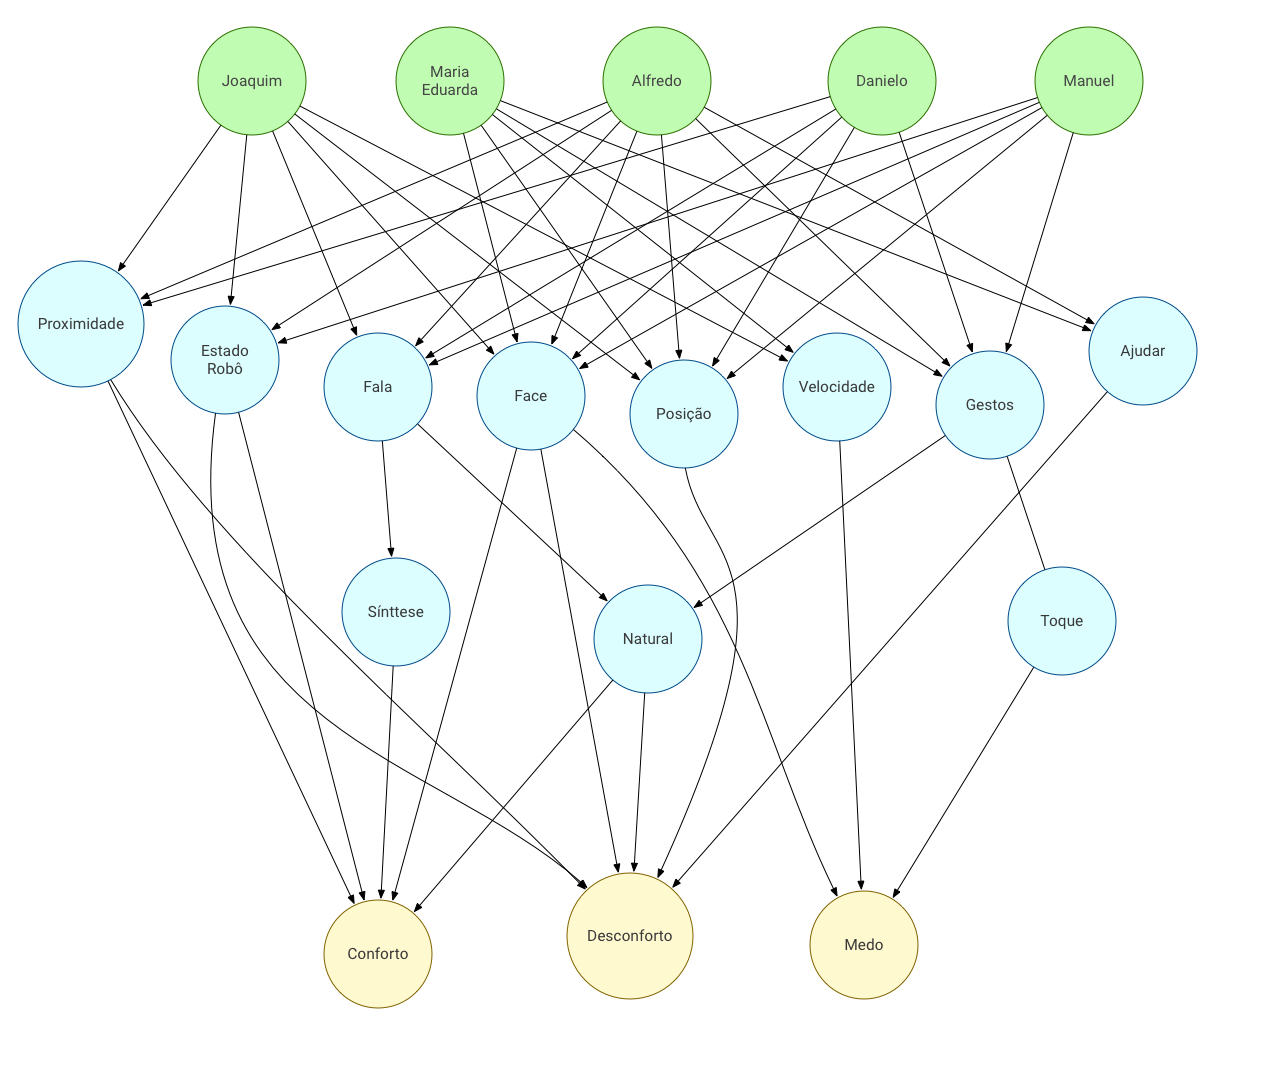
\includegraphics[width=\textwidth]{rb-thesis.png}
		\smallcaption{Fonte: Autor.}
		\label{fig:rb}
	\end{minipage}
\end{figure}

A rede bayesiana da figura~\ref{fig:rb} funciona da seguinte maneira, são fixados os valores de evidência nos nós folha (amarelos) e nos nós internos (azuis). Com base nas evidências apresentadas, a rede responde a probabilidade de ser cada uma das Personas que compõem os nós raizes (verdes). A partir da classificação é possível identificar qual o perfil do usuário, em interação com o robô. É importante ressaltar que a classificação do usuário é feita com base em sua experiência, pois é o principal interessado na interação com o robô. A grande preocupação em manter o foco no ser humano é por que ele é o mais interassado na interação com o sistema. A tomada de decisão para melhorar a experiência do usuário a partir da classificação do perfil do usuário pelo robô não faz parte do escopo desta tese. Porém nas seções a seguir são apresentados os passos para definir os valores de probabilidades condicionais, consumir, extrair conhecimento e evoluir o classificador a partir da base apresentada nessa seção.

\section{Definindo os valores de probabilidades condicionais}
\label{sec:tpc}
Com a estrutura da rede bayesiana definida, antes de utilizá-la para classificar as Personas, é necessário definir as tabelas com os valores das probabilidades condicionais para cada variável. Para construir as tabelas de probabilidades condicionais~(TPC), é feito a análise das respostas nos questionários e sobre as anotações realizados durante o teste de interação. Durante o processo de análise é identificado a frequência dos eventos que envolvem cada variável. A partir da contabilidade dos eventos utilizam-se as equações de teoria de probabilidade apresentadas ao longo da seção~\ref{sec:raciocinio-probabilistico}. As equações devolvem os valores das probabilidades de acordo com os eventos observados. Todos os valores são normalizados para manter a somatória das probabilidades igual a 1. Na sequência, o processo de consumo da rede bayesiana é descrito para auxiliar na classificação do perfil do usuário como Persona.

\section{Executando a classificação da Persona}
\label{sec:consumo}
Para classificar a Persona, é necessário implementar o cálculo das propabilidades condicionais no robô. Com a implementação concluída é realizado a interação do robô, onde é capturado as evidências das variáveis que auxiliam a determinar os valores de cada variável da camada interna e também da camada folha da rede bayesiana.

O resultado a partir das evidências identificadas durante a interação, é a probabilidade de cada Persona ser enquadrada pelo perfil daquele usuário. Para definir a Persona, deve-se identificar qual delas têm a maior probabilidade de ser classificada como similar ao perfil do usuário. Nessa tese, para efeito de visualização da rede bayesiana, utilizou-se um programa chamado SamIam~\footnote{http://reasoning.cs.ucla.edu/samiam/}. Ele é capaz de criar e executar uma rede bayesiana através de uma interface visual, facilitando identificar o comportamento dela. A figura~\ref{fig:samiam} apresenta a interface do programa SamIam.

\begin{figure}[ht!]
	\centering
	\begin{minipage}{\textwidth}
		\caption{Rede bayesiana implementada no programa SamIam.}
		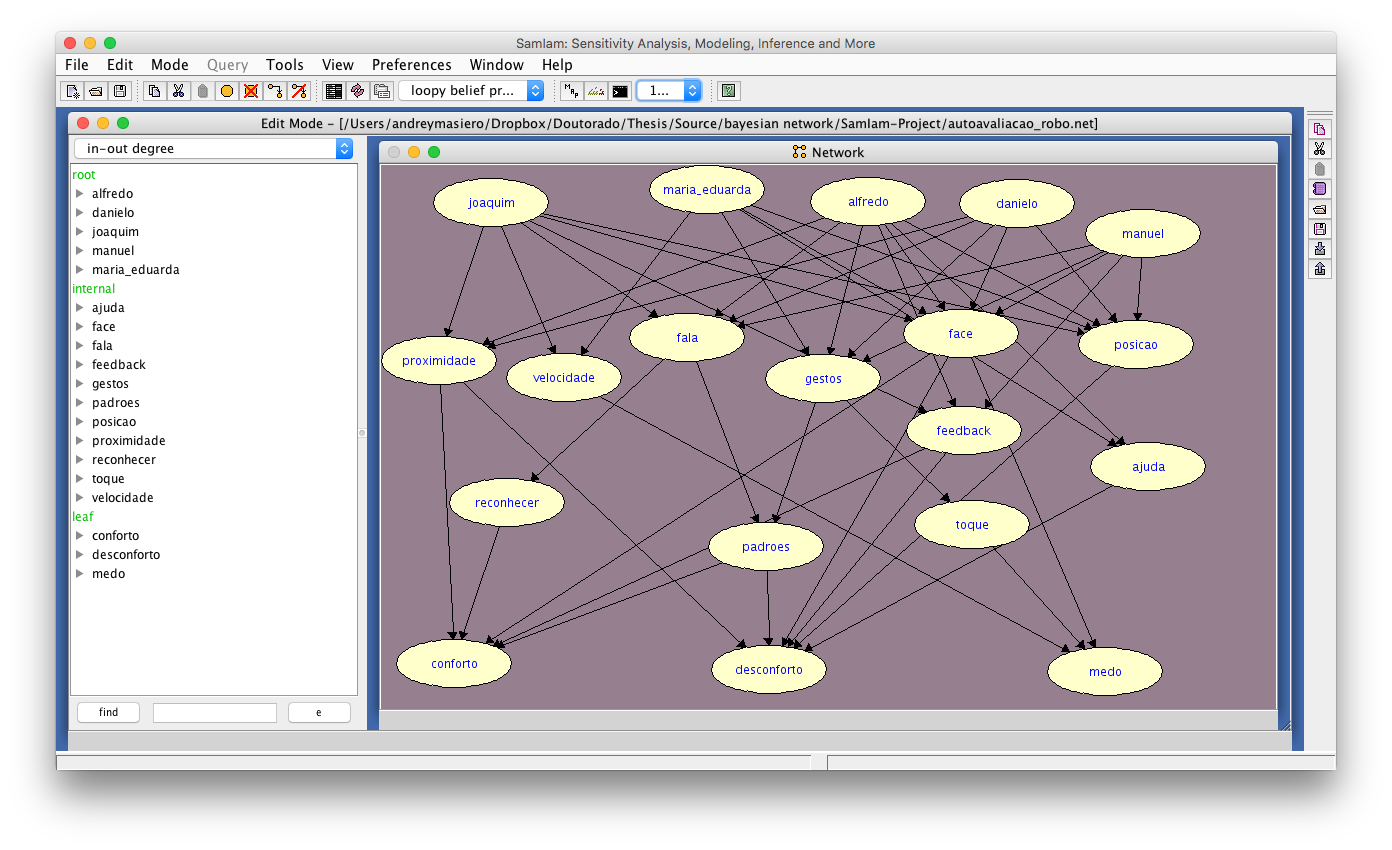
\includegraphics[width=\textwidth]{samiam.png}
		\smallcaption{Fonte: Autor.}
		\label{fig:samiam}
	\end{minipage}
\end{figure}

Na figura~\ref{fig:samiam} é apresentado a implementação da rede bayesiana estrutura na figura~\ref{fig:rb}. Nele é possível monitorar as variáveis que representam as Personas e, ao alterar os valores das variáveis de evidência e saber qual o perfil com maior probabilidade. A identificação das variáveis é discutida na seção~\ref{sec:idvariavel}, a seguir.

\section{Identificando as variáveis de interação}
\label{sec:idvariavel}
As variáveis referentes as Personas são dadas a partir da consulta a rede bayesiana. As demais variáveis são capturadas por outras fontes de informação. As variáveis de ações do robô e heurísticas, são capturadas a partir do comportamento programado para realizar a tarefa. A variável proximidade é capturada através dos sensores de distância como Microsoft\textregistered\ Kinect\textregistered\ e o \emph{laser} Hokuyo URG-04. O primeiro é possível rastrear o esqueleto virtual do usuário e determinar a distância através de uma transformada geométrica. O segundo mensura a distância de qualquer objeto na direção da base do robô. Assim, é possível verificar a distância dos pés dos usuário.

A variável sobre a posição do usuário é também capturada através do sensor de movimento e distância Microsoft\textregistered\ Kinect\textregistered. A partir das informações retornadas do esqueleto virtual, comparando a altura das articulações do joelho, com o quadril da pessoa. Por fim, as variáveis comportamentais devem ser capturadas. As variáveis comportamentais que foram consideradas na construção da rede bayesiana foram: conforto, desconforto e medo. Nessa tese, as variáveis comportamentais foram capturadas pela declaração do usuário, onde ele informava o que estava sentido com o robô e essa informação era inserida manualmente no mecanismo de classificação. Contudo, essas informações podem ser capturadas automaticamente. Para isso, é necessário definir como são identificados cada variável comportamental e criar componentes capazes de detectá-las.

Com todos os componentes para identificar as variáveis existentes na rede bayesiana, basta realizar a consulta a partir da evidência sobre o que ocorreu na interação. Assim, a classificação do usuário é realizada e o robô pode efetuar uma adaptação de suas ações na interação. A adaptação das ações do robô são discutidas a seguir, na seção~\ref{sec:classificapersona}

\section{Adaptando as ações do robô de acordo com a Persona}
\label{sec:classificapersona}
Após a execução da consulta na rede bayesiana, as Personas que possuem probabilidade de serem similar ao perfil do usuário são identificadas. O sistema deve selecionar a Persona que possui a maior probabilidade de ser o perfil, para seguir a adaptação das ações do robô. Com a Persona identificada, é importante acionar um mecanismo de tomada de decisão que controla as ações do robô de maneira a aumentar o conforto da pessoa na interação e diminuir o desconforto e o medo. Existem diversas técnicas que podem ser aplicadas nesse passo, por exemplo, Árvores de Decisão, Raciocinio Baseado em Casos, Aprendizado por Reforço, métodos probabilísticos, entre outros. Contudo, a adaptação das ações do robô através de mecanismos de tomada de decisão, não fazem parte do escopo desta tese. No capítulo~\ref{cap:evolucao} é apresentado os passos para evoluir o classificador e também o projeto de IHR apresentados até o momento.
